\chapter{Geschwindigkeitsaddition, Lichtkegel und Vierervektoren}

\section{Zwei Bezugssysteme auf einem Eisenbahngleis}

Die zuvor hergeleitete Lorentz-Transformation bezog sich auf eine bewusst eingeschränkte Geometrie: Jede Relativbewegung verlief entlang einer Achse. Stellen Sie sich ein langes Eisenbahngleis vor. Eine Gruppe von Beobachtern bleibt am Bahnhof, eine andere fährt in einem Zug, der sich entlang des Gleises bewegt. Die transversalen Richtungen sind vorhanden, spielen aber erst eine Rolle, wenn sie später wieder einbezogen werden.

Jedes Bezugssystem ist ein operational definiertes Koordinatensystem. Im Bezugssystem ruhende Meterstäbe legen die räumlichen Koordinaten fest, und dort ruhende, synchronisierte Uhren legen die Zeit fest. Das Postulat, das ihren Zusammenhang bestimmt, besagt, dass alle Inertialbeobachter dieselbe Lichtgeschwindigkeit messen.

Die meisten Rechnungen verwenden \(c=1\). Die Zeit kann in Sekunden und die Entfernung in Lichtsekunden oder in Jahren und Lichtjahren gemessen werden. Geschwindigkeiten sind dann dimensionslose Bruchteile der Lichtgeschwindigkeit. Werden gewöhnliche Einheiten benötigt, ergeben sich die Faktoren \(c\) durch Dimensionskonsistenz eindeutig; zum Beispiel wird \(v^2\) in einem dimensionslosen Lorentzfaktor zu \(v^2/c^2\).

\subsection{Direkte und inverse Transformationen}

Ein Lichtblitz ereigne sich irgendwo im Zug oder in seiner Nähe. Es ist ein Ereignis, unabhängig davon, wer es beschreibt. Der Beobachter am Bahnhof ordnet ihm \((x,t)\) zu, der Beobachter im Zug dagegen \((x',t')\). In den Einheiten \(c=1\) gilt
\begin{align}
x'&=\gamma_v(x-vt),&
t'&=\gamma_v(t-vx),
\label{eq:sr2-direct}\\
\gamma_v&=\frac{1}{\sqrt{1-v^2}}.
\end{align}
Die Verschiebung \(x-vt\) wäre Newton vertraut; der Faktor \(\gamma_v\) und die Beimischung von \(x\) zu \(t'\) sind die relativistischen Änderungen.

\begin{figure}[htbp]
\centering
\includegraphics[width=0.90\textwidth]{lecture_02_figure_01.png}
\caption{Die direkte Lorentz-Transformation, die die Bahnhofkoordinaten \((x,t)\) mit den Zugkoordinaten \((x',t')\) verknüpft.}
\lectureframe{00:07:52}
\end{figure}

Aus der Reziprozität ergibt sich die inverse Transformation, indem man das Vorzeichen der Relativgeschwindigkeit umkehrt:
\begin{align}
x&=\gamma_v(x'+vt'),&
t&=\gamma_v(t'+vx').
\label{eq:sr2-inverse}
\end{align}
Der Bahnhof ist nicht absolut in Ruhe. Er ist lediglich das Bezugssystem, das ungestrichene Koordinaten erhält; aus Sicht des Zuges bewegt er sich mit \(-v\).

\begin{figure}[htbp]
\centering
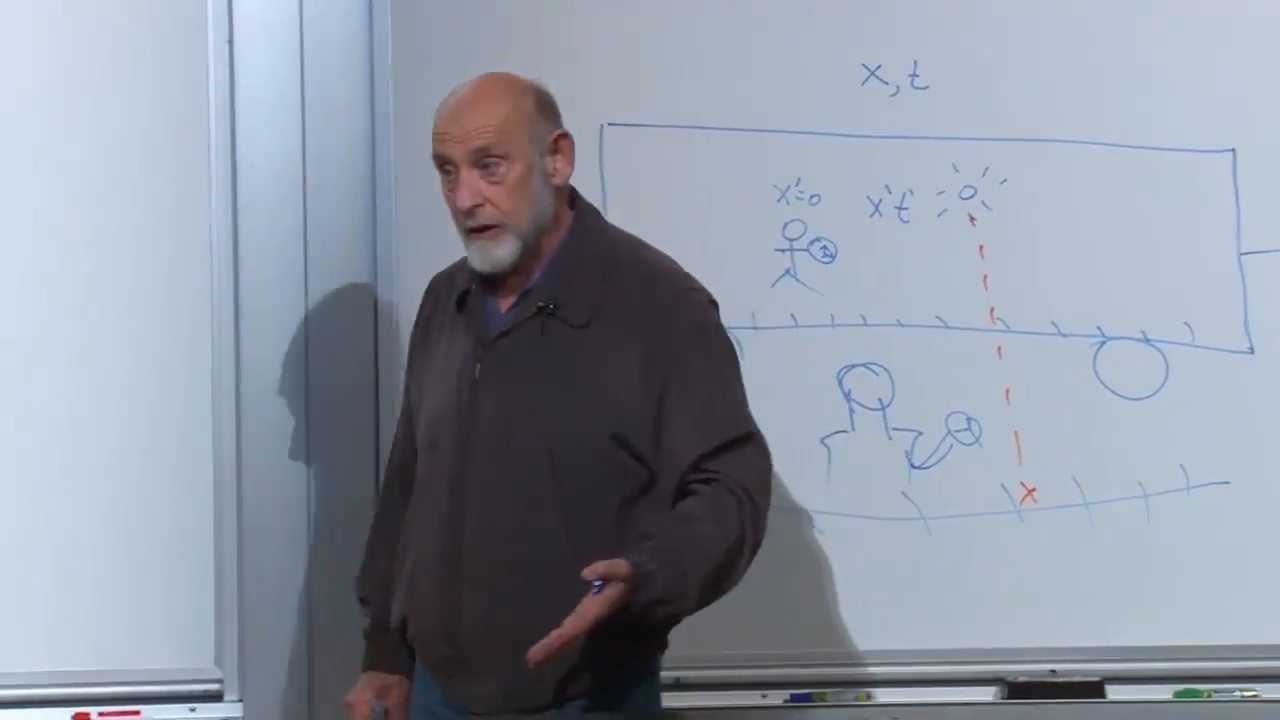
\includegraphics[width=0.90\textwidth]{lecture_02_figure_02.png}
\caption{Die inverse Abbildung hat denselben Lorentzfaktor und das entgegengesetzte Vorzeichen der Relativgeschwindigkeit.}
\lectureframe{00:09:15}
\end{figure}

Bei einem Boost entlang \(x\) ändern sich die transversalen Koordinaten nicht:
\begin{equation}
y'=y,
\qquad
z'=z.
\end{equation}

Die Relativgeschwindigkeit lässt sich aus der Ortsgleichung ablesen, ohne ihren Nenner zu betrachten. Der Zugursprung ist durch \(x'=0\) definiert, also gilt
\begin{equation}
x'=0
\quad\Longleftrightarrow\quad
x-vt=0
\quad\Longleftrightarrow\quad
x=vt.
\label{eq:sr2-origin-worldline}
\end{equation}
Der Koeffizient von \(t\) in dieser Weltlinie ist die Geschwindigkeit des Zuges in den Bahnhofkoordinaten.

\section{Drei Bezugssysteme und die Zusammensetzung von Boosts}

Stellen Sie ein kleines Tretauto in den Zug. Der Zug bewegt sich relativ zum Bahnhof mit der Geschwindigkeit \(v\), während sich das Auto relativ zum Fahrgast mit der Geschwindigkeit \(u\) den Gang entlang bewegt. Die Geschwindigkeit des Autos relativ zum Bahnhof sei \(w\). Nach Newtonscher Intuition wäre \(w=u+v\), doch die Lorentz-Transformationen müssen die Entscheidung liefern.

Nun gibt es drei Koordinatensysteme:
\begin{equation}
(x,t),\qquad (x',t'),\qquad (x'',t'').
\end{equation}
Das erste gehört zum Bahnhof, das zweite zum Zug und das dritte zum Auto. Zwischen Zug und Auto gilt
\begin{align}
x''&=\gamma_u(x'-ut'),&
t''&=\gamma_u(t'-ux'),
\label{eq:sr2-second-boost}\\
\gamma_u&=\frac{1}{\sqrt{1-u^2}}.
\end{align}

\begin{figure}[htbp]
\centering
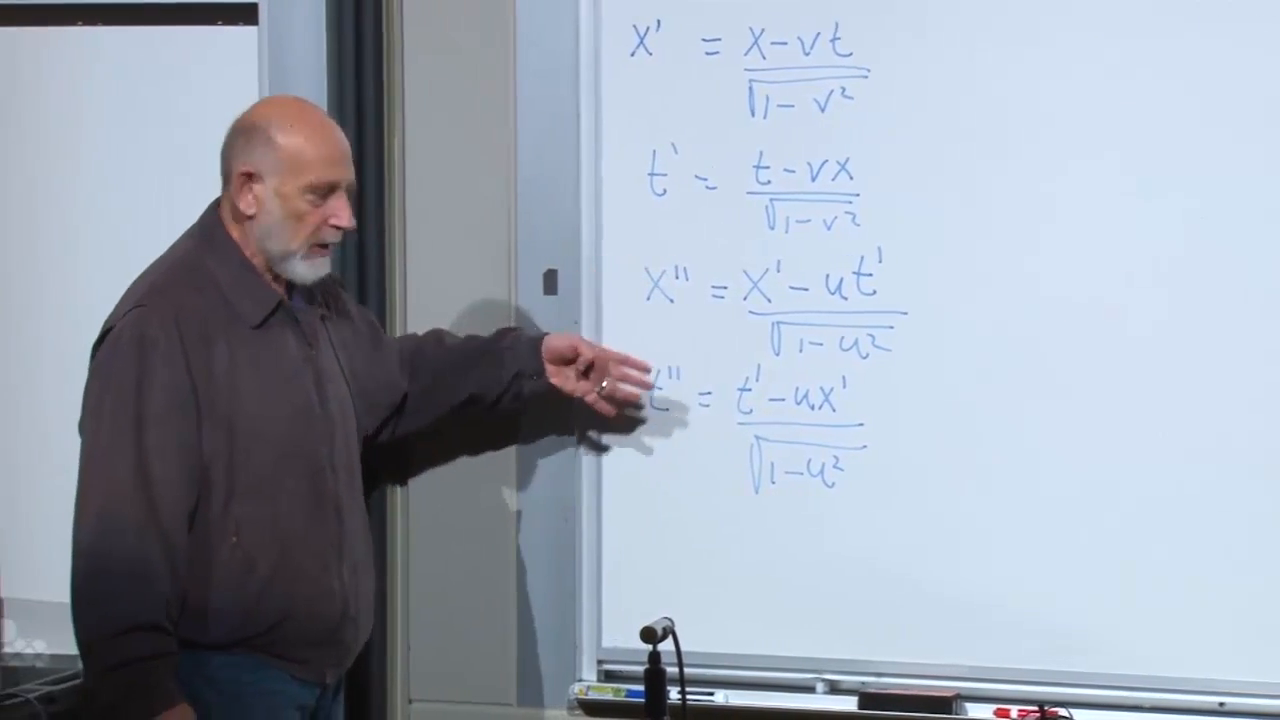
\includegraphics[width=0.90\textwidth]{lecture_02_figure_03.png}
\caption{Auf die direkten Formeln vom Bahnhof zum Zug folgt eine zweite Lorentz-Transformation von gestrichenen zu doppelt gestrichenen Koordinaten.}
\lectureframe{00:14:55}
\end{figure}

\subsection{Einen Boost in den anderen einsetzen}

Um \(w\) zu bestimmen, genügt die Ortsgleichung. Setzen Sie \eqref{eq:sr2-direct} in die erste Gleichung von \eqref{eq:sr2-second-boost} ein:
\begin{align}
x''
&=\gamma_u(x'-ut')\\
&=\gamma_u\gamma_v\left[(x-vt)-u(t-vx)\right]\\
&=\gamma_u\gamma_v\left[(1+uv)x-(u+v)t\right].
\label{eq:sr2-composed-space}
\end{align}
Die beiden Minuszeichen im Term \(uvx\) ergeben ein Pluszeichen; die beiden Zeitanteile fassen sich zu \(-(u+v)t\) zusammen.

\begin{figure}[htbp]
\centering
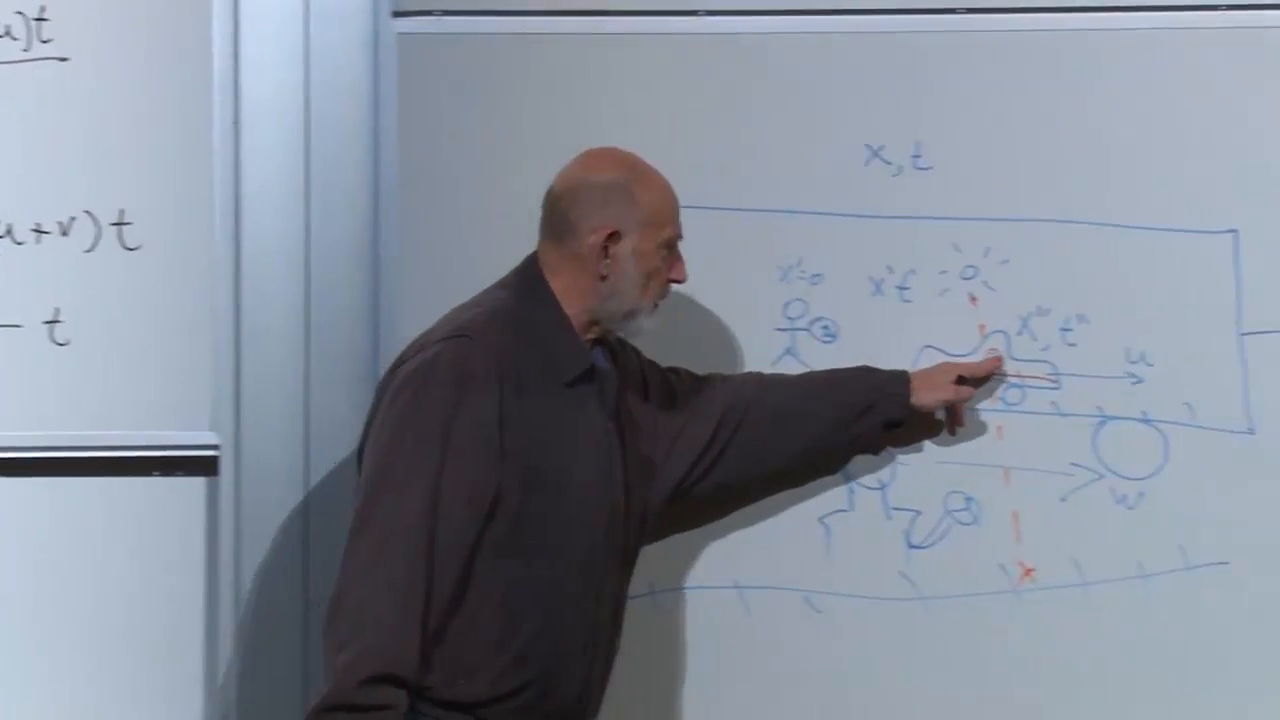
\includegraphics[width=0.91\textwidth]{lecture_02_figure_04.png}
\caption{Die verschachtelte Einsetzung vor dem Zusammenfassen der Terme mit \(x\) und \(t\) im zusammengesetzten Boost.}
\lectureframe{00:16:30}
\end{figure}

Wie zuvor ist der Nenner für die Bestimmung des bewegten Ursprungs unerheblich. Das Tretauto ruht bei \(x''=0\), daher muss die Klammer in \eqref{eq:sr2-composed-space} verschwinden:
\begin{equation}
(1+uv)x-(u+v)t=0.
\end{equation}
Seine Weltlinie im Bahnhofsystem lautet daher
\begin{equation}
x=\frac{u+v}{1+uv}\,t,
\end{equation}
und seine Geschwindigkeit ist
\begin{equation}
\boxed{w=\frac{u+v}{1+uv}}.
\label{eq:sr2-velocity-add-c1}
\end{equation}

\begin{figure}[htbp]
\centering
\includegraphics[width=0.91\textwidth]{lecture_02_figure_05.png}
\caption{Der zusammengefasste Zähler und die Weltlinie \(x=[(u+v)/(1+uv)]t\) geben die zusammengesetzte Geschwindigkeit zu erkennen.}
\lectureframe{00:19:30}
\end{figure}

Auch die Zeitgleichung lässt sich konsistent zusammensetzen. Die vollständige Transformation vom Bahnhof zum Auto hat die Lorentz-Form
\begin{align}
x''&=\gamma_w(x-wt),&
t''&=\gamma_w(t-wx),
\end{align}
mit
\begin{equation}
\gamma_w=\frac{1}{\sqrt{1-w^2}}.
\end{equation}
Tatsächlich gilt
\begin{equation}
\gamma_w=\gamma_u\gamma_v(1+uv),
\end{equation}
Dies folgt, wenn man \eqref{eq:sr2-velocity-add-c1} einsetzt und vereinfacht. Zwei kollineare Boosts ergeben also zusammen wieder einen kollinearen Boost.

\subsection{Dimensionen wiederherstellen}

\begin{classroomqa}
\audiencequestion{Warum ist der Nenner \(1+uv\) in gewöhnlichen Einheiten dimensionswidrig?}
\lecturerresponse{Er ist nur deshalb korrekt, weil \(c=1\) jede Geschwindigkeit zu einem dimensionslosen Bruchteil der Lichtgeschwindigkeit macht. In konventionellen Einheiten muss das Produkt als \(uv/c^2\) auftreten und ist dann dimensionslos. \lecturetimestamp{00:21:11}}
\end{classroomqa}

Das dimensionsbehaftete Gesetz der Geschwindigkeitsaddition lautet
\begin{equation}
\boxed{
w=\frac{u+v}{1+\dfrac{uv}{c^2}}
}.
\label{eq:sr2-velocity-add}
\end{equation}

\begin{figure}[htbp]
\centering
\includegraphics[width=0.90\textwidth]{lecture_02_figure_06.png}
\caption{Aufgrund der Dimensionskonsistenz tritt unter dem Produkt \(uv\) der Faktor \(c^2\) auf.}
\lectureframe{00:22:06}
\end{figure}

Für \(\lvert u\rvert,\lvert v\rvert\ll c\) gilt
\begin{equation}
\frac{uv}{c^2}\ll 1,
\end{equation}
also
\begin{equation}
w\approx u+v.
\end{equation}
Die Newtonsche Addition ist die Näherung für kleine Geschwindigkeiten und keine eigenständige Regel.

\subsection{Zwei numerische Bereiche}

Betrachten wir zunächst
\begin{equation}
u=v=0.01c.
\end{equation}
In den Einheiten \(c=1\) gilt
\begin{equation}
w=\frac{0.02}{1.0001}\approx 0.019998.
\end{equation}
Ein Prozent der Lichtgeschwindigkeit entspricht bereits ungefähr \(3\times10^6\ {\rm m/s}\), dennoch beträgt die relativistische Korrektur nur ein Zehntausendstel. Das Ergebnis ist geringfügig kleiner als die Newtonsche Vorhersage \(0.02c\).

\begin{figure}[htbp]
\centering
\includegraphics[width=0.90\textwidth]{lecture_02_figure_07.png}
\caption{Bei \(u=v=0.01c\) weicht der Nenner nur um \(10^{-4}\) von eins ab.}
\lectureframe{00:24:23}
\end{figure}

Betrachten wir nun
\begin{equation}
u=v=0.9c.
\end{equation}
Nach Newton ergäbe sich \(1.8c\). Die Relativitätstheorie liefert
\begin{equation}
\frac{w}{c}
=\frac{0.9+0.9}{1+0.9^2}
=\frac{1.8}{1.81}
\approx 0.9945.
\label{eq:sr2-fast-example}
\end{equation}

\begin{figure}[htbp]
\centering
\includegraphics[width=0.90\textwidth]{lecture_02_figure_08.png}
\caption{Zwei Geschwindigkeiten von \(0.9c\) ergeben zusammen \(1.8/1.81\), also weiterhin weniger als die Lichtgeschwindigkeit.}
\lectureframe{00:25:48}
\end{figure}

Aufeinanderfolgende unterluminale Boosts können die Lichtgeschwindigkeit \(c\) nicht überschreiten. Wenn \(u<c\) und \(v<c\) gelten, dann gilt
\begin{equation}
1-\frac{w}{c}
=
\frac{\left(1-\frac{u}{c}\right)
      \left(1-\frac{v}{c}\right)}
     {1+\frac{uv}{c^2}}
>0.
\end{equation}
Jeder weitere Boost kann das Ergebnis näher an \(c\) heranbringen, aber niemals darüber hinaus. Für den Grenzwert \(u=c\) gilt
\begin{equation}
w=\frac{c+v}{1+v/c}=c.
\end{equation}
Die Lichtgeschwindigkeit ist ein Fixpunkt des Zusammensetzungsgesetzes.

\section{Koordinatenmessung ist nicht gleich visuelle Erscheinung}

\begin{classroomqa}
\audiencequestion{Wenn der Zug Glaswände hat, könnte der Beobachter am Bahnhof den Fahrgast und das Tretauto dann nicht einfach gemeinsam ansehen und ihre Bewegungen direkt ablesen?}
\lecturerresponse{Die Lorentz-Transformation bezieht sich auf Koordinatenmessungen mit räumlich verteilten Maßstäben und synchronisierten Uhren. Ein visuelles Bild enthält außerdem die unterschiedlichen Laufzeiten des Lichts von verschiedenen Ereignissen bis zum Beobachter. Glas verändert den Anblick, nicht den Koordinatenzusammenhang; ein einzelnes Bild als gleichzeitige Daten zu behandeln, würde genau jene Gleichzeitigkeit voraussetzen, die durch die Relativitätstheorie korrigiert wurde. \lecturetimestamp{00:27:53}}
\end{classroomqa}

Ein Ereignis hat in jedem Bezugssystem einen Ort und eine Zeit, unabhängig davon, ob es gerade jemand sieht. Die optische Erscheinung ist ein legitimer Untersuchungsgegenstand, erfordert aber eine zweite Rechnung, die das Licht von jedem Ereignis bis zum Auge verfolgt. Die Transformationsgesetze selbst sind universell und unabhängig von den Wänden des Zuges.

\section{Das Eigenintervall in drei räumlichen Dimensionen}

Kehren wir zu zwei Ereignissen zurück: Das eine liegt zunächst im Ursprung, das andere bei \((x,t)\). In einer räumlichen Dimension gilt
\begin{equation}
\tau^2=t^2-x^2
\label{eq:sr2-interval-1d}
\end{equation}
in den Einheiten \(c=1\). Alle Inertialsysteme stimmen überein:
\begin{equation}
\tau^2
=t^2-x^2
=t'^2-x'^2
=t''^2-x''^2.
\end{equation}
Die Koordinaten ändern sich, das Eigenintervall bleibt unverändert.

Bei zeitartiger Trennung kann sich eine Uhr zwischen den Ereignissen bewegen. Zeigt sie beim ersten Ereignis Mittag an, so ist die verstrichene Zeit bis zum zweiten Ereignis die Eigenzeit \(\tau\). Diese Aussage ist unabhängig davon, welches Koordinatensystem zur Berechnung des Intervalls verwendet wird.

\begin{figure}[htbp]
\centering
\includegraphics[width=0.90\textwidth]{lecture_02_figure_09.png}
\caption{Zur Erinnerung die invariante Eigenzeitbeziehung \(\tau^2=t^2-x^2\), bevor die transversalen Richtungen wieder einbezogen werden.}
\lectureframe{00:30:18}
\end{figure}

\subsection{Die transversalen Richtungen durch räumliche Drehungen wieder einbeziehen}

Betrachten wir eine gewöhnliche Drehung der räumlichen Achsen, bevor wir zu Boosts zurückkehren. Für einen Punkt, der nicht auf der \(x\)-Achse liegt, beträgt das Quadrat des räumlichen Abstands
\begin{equation}
r^2=x^2+y^2+z^2,
\end{equation}
und bleibt nach dem gewöhnlichen Satz des Pythagoras bei Drehungen invariant. Das \(3+1\)-dimensionale Raumzeitintervall lautet folglich
\begin{equation}
\boxed{
\tau^2=t^2-x^2-y^2-z^2
}.
\label{eq:sr2-interval-3d}
\end{equation}
Mit wiederhergestelltem \(c\) gilt
\begin{equation}
c^2\tau^2
=c^2t^2-x^2-y^2-z^2.
\end{equation}

\begin{figure}[htbp]
\centering
\includegraphics[width=0.90\textwidth]{lecture_02_figure_10.png}
\caption{Der Satz des Pythagoras für den räumlichen Abstand erweitert die Invariante von \(t^2-x^2\) auf \(t^2-x^2-y^2-z^2\).}
\lectureframe{00:34:23}
\end{figure}

Jede Kombination aus räumlichen Drehungen und Lorentz-Boosts lässt \eqref{eq:sr2-interval-3d} invariant. Gewöhnliche Koordinatenachsen können sich über die Komponenten uneinig sein, stimmen aber im euklidischen Abstand überein; Inertialsysteme der Raumzeit können sich über die Raum- und Zeitkomponenten uneinig sein, stimmen aber in dieser Differenz der Quadrate überein. Diese Invariante ist die zentrale geometrische Tatsache der speziellen Relativitätstheorie.

\begin{classroomqa}
\audiencequestion{Erhalten Beobachter im Zug und am Bahnhof dieselbe Lichtgeschwindigkeit, wenn der Fahrgast das Tretauto durch einen nach vorn gerichteten Lichtstrahl ersetzt?}
\lecturerresponse{Setzen Sie \(u=c\) in \eqref{eq:sr2-velocity-add} ein. Dann gilt \(w=(c+v)/(1+v/c)=c\). In den Einheiten \(c=1\) ist das Verhältnis einfach \((1+v)/(1+v)=1\). Beide Bezugssysteme messen dieselbe Geschwindigkeit, genau wie gefordert. \lecturetimestamp{00:35:53}}
\end{classroomqa}

Die frühere Frage zu den Glaswänden zeigt also keinen Fehler bei der Invarianz der Lichtgeschwindigkeit. Sie beruht auf einer Verwechslung von Koordinatenmessung und verzögertem visuellem Bild, letztlich auf einer Verwechslung hinsichtlich der Gleichzeitigkeit.

\section{Nullstrahlen und der Lichtkegel}

In einer Raumdimension erfüllen nach rechts und links laufende Lichtstrahlen
\begin{equation}
x=\pm t.
\end{equation}
Ihr Intervall verschwindet:
\begin{equation}
t^2-x^2=0.
\end{equation}
Anders als beim euklidischen Abstand bedeutet ein verschwindendes Raumzeitintervall nicht, dass die Ereignisse zusammenfallen. Es bedeutet, dass ein Lichtsignal sie miteinander verbinden kann.

Wenn alle räumlichen Richtungen einbezogen werden, gilt für einen Lichtstrahl
\begin{equation}
t^2-x^2-y^2-z^2=0,
\label{eq:sr2-null}
\end{equation}
oder
\begin{equation}
r=t
\end{equation}
für zukunftsgerichtetes Licht in den Einheiten \(c=1\).

\begin{figure}[htbp]
\centering
\includegraphics[width=0.90\textwidth]{lecture_02_figure_11.png}
\caption{Licht breitet sich in jeder räumlichen Richtung entlang einer Nulltrajektorie aus, die \(t^2-(x^2+y^2+z^2)=0\) erfüllt.}
\lectureframe{00:39:28}
\end{figure}

In \(1+1\) Dimensionen besteht die Nullmenge aus einem Paar von Geraden mit einem Winkel von \(45^\circ\). Mit zwei Raumdimensionen und einer Zeitdimension wird daraus ein Kegel; drei Raumdimensionen lassen sich nicht vollständig an einer Tafel darstellen, doch die definierende Gleichung bleibt unverändert.

Der zukünftige Lichtkegel umfasst die Ereignisse, die das am Ursprung ausgesandte Licht erreichen kann. Der vergangene Lichtkegel umfasst die Ereignisse, von denen Licht den Ursprung erreichen kann. Der eine entsteht aus dem anderen durch eine Umkehrung der Zeitrichtung.

\begin{figure}[htbp]
\centering
\includegraphics[width=0.90\textwidth]{lecture_02_figure_12.png}
\caption{Die Nullstrahlen bei \(45^\circ\) bilden in einer höherdimensionalen Raumzeitdarstellung den zukünftigen und den vergangenen Lichtkegel.}
\lectureframe{00:40:47}
\end{figure}

\begin{classroomqa}
\audiencequestion{Welche Größe ist in der Newtonschen Mechanik unter Galilei-Transformationen invariant?}
\lecturerresponse{Das Zeitintervall selbst. Alle Newtonschen Beobachter stimmen über \(\Delta t\) überein, auch wenn sie sich über die räumliche Verschiebung uneinig sind. Die Relativitätstheorie gibt die universelle Zeit auf und ersetzt sie durch das invariante Raumzeitintervall. \lecturetimestamp{00:41:53}}
\end{classroomqa}

\section{Von räumlichen Vektoren zu Vierervektoren}

Die hier betrachteten Vektoren sind geometrische Vektoren, keine Quantenzustandsvektoren. Eine Verschiebung zwischen zwei Punkten im gewöhnlichen Raum hat einen Betrag und eine Richtung. Man kann ihren Anfangspunkt zum Ursprung verschieben, ohne den Vektor zu ändern, und ihre drei Komponenten bezeichnen mit
\begin{equation}
x^i=(x^1,x^2,x^3)=(x,y,z),
\qquad i=1,2,3.
\end{equation}
Der lateinische Index \(i\) läuft nur über die räumlichen Richtungen.

Ein Ereignis benötigt eine zusätzliche Komponente: seine Zeit. Eine Raumzeitposition schreibt man daher als
\begin{equation}
x^\mu=(x^0,x^1,x^2,x^3)=(t,x,y,z),
\qquad \mu=0,1,2,3.
\label{eq:sr2-four-position}
\end{equation}
Historisch bedingt ist die Zeit die nullte statt der vierten Komponente:
\begin{equation}
x^0=t,\qquad x^1=x,\qquad x^2=y,\qquad x^3=z.
\end{equation}
Griechische Indizes wie \(\mu\) laufen über die Raumzeit; lateinische Indizes wie \(i\) über den Raum.

\begin{figure}[htbp]
\centering
\includegraphics[width=0.90\textwidth]{lecture_02_figure_13.png}
\caption{Die räumlichen Komponenten \(x^i\) werden zur vierkomponentigen Raumzeitposition \(x^\mu=(x^0,x^1,x^2,x^3)\) erweitert.}
\lectureframe{00:46:05}
\end{figure}

Die Invariante lautet nun
\begin{equation}
\tau^2
=(x^0)^2-(x^1)^2-(x^2)^2-(x^3)^2.
\end{equation}
Die Notation allein fügt keine neue Physik hinzu. Ihr Vorteil besteht darin, dass eine Lorentz-Transformation linear auf alle vier Komponenten wirkt, so wie eine Drehung linear auf einen räumlichen Vektor wirkt.

\begin{classroomqa}
\audiencequestion{Kann eine lineare Transformation als Matrix dargestellt werden, die auf einen Spaltenvektor wirkt?}
\lecturerresponse{Ja. Bei einem Boost entlang \(x\) wirkt der nichttriviale Block \(\gamma_v\begin{pmatrix}1&-v\\-v&1\end{pmatrix}\) auf \((t,x)^{\mathsf T}\), während \(y\) und \(z\) unverändert bleiben. Die Matrixnotation ist die natürliche Art, Lorentz-Transformationen zusammenzusetzen und zu ordnen. \lecturetimestamp{00:48:14}}
\end{classroomqa}

Explizit gilt
\begin{equation}
\begin{pmatrix}
t'\\x'\\y'\\z'
\end{pmatrix}
=
\begin{pmatrix}
\gamma_v&-\gamma_v v&0&0\\
-\gamma_v v&\gamma_v&0&0\\
0&0&1&0\\
0&0&0&1
\end{pmatrix}
\begin{pmatrix}
t\\x\\y\\z
\end{pmatrix}.
\label{eq:sr2-boost-matrix}
\end{equation}

\section{Verschiebungen und Vierergeschwindigkeit}

Gehen wir von der Position eines Ereignisses zu einem kurzen Abschnitt der Weltlinie eines Teilchens über. Die Viererverschiebung ist
\begin{equation}
\Delta x^\mu
=(\Delta t,\Delta x,\Delta y,\Delta z).
\end{equation}
Wenn eine Verschiebung als klein bezeichnet wird, kommt die Differentialrechnung ins Spiel: Aus \(\Delta x^\mu\) wird \(dx^\mu\). Vorerst macht die endliche Schreibweise die Geometrie anschaulich.

Das Eigenzeitintervall entlang einer zeitartigen Weltlinie erfüllt
\begin{equation}
(\Delta\tau)^2
=(\Delta t)^2-(\Delta x)^2-(\Delta y)^2-(\Delta z)^2.
\label{eq:sr2-proper-increment}
\end{equation}
Die gewöhnliche Geschwindigkeit ist die räumliche Verschiebung geteilt durch die Koordinatenzeit und hat drei Komponenten. Die Vierergeschwindigkeit hingegen ist die Viererverschiebung geteilt durch die invariante Eigenzeit:
\begin{equation}
u^\mu
=\frac{\Delta x^\mu}{\Delta\tau}
\quad\longrightarrow\quad
\boxed{
u^\mu=\frac{dx^\mu}{d\tau}
}.
\label{eq:sr2-four-velocity}
\end{equation}

\begin{figure}[htbp]
\centering
\includegraphics[width=0.90\textwidth]{lecture_02_figure_14.png}
\caption{Ein Weltlinienabschnitt legt \(\Delta x^\mu\), die invariante Größe \(\Delta\tau\) und die Vierergeschwindigkeit \(u^\mu=\Delta x^\mu/\Delta\tau\) fest.}
\lectureframe{00:52:42}
\end{figure}

Dieses Objekt hat vier Komponenten und transformiert sich wie ein Vierervektor. Wie es mit der gewöhnlichen Dreiergeschwindigkeit zusammenhängt, ist die nächste Frage, die hier bewusst offenbleibt. Ihre Klärung führt zur relativistischen Impuls-, Energie- und Beschleunigungslehre und schließlich zur relativistischen Verallgemeinerung von \(F=ma\).